\chapter{Una novedosa forma de crear Apps: Apache Cordova}
\section{Pasos para instalar el proyecto}
\begin{enumerate}
    \item Clonar el proyecto \href{https://github.com/rgaluppo/runtime_permissions_test}{runtime-permissions-test}.
    \item Agregar plugins
        \begin{lstlisting}[style=BashInputStyle]
          $ cordova plugin add cordova.plugins.diagnostic@3.0
          $ cordova plugin add cordova-plugin-calendar
          $ cordova plugin add cordova-plugin-contacts
          $ cordova plugin add cordova-plugin-geolocation
          $ cordova plugin add cordova-sms-plugin
        \end{lstlisting}
    \item Agregar plataforma seg\'un corresponda
        \begin{lstlisting}[style=BashInputStyle]
          $ cordova platform add ios
        \end{lstlisting}
                \begin{lstlisting}[style=BashInputStyle]
          $ cordova platform add android
        \end{lstlisting}
    \item Correr la m\'aquina virtual seg\'un la plataforma elegida en el paso anterior
        \begin{lstlisting}[style=BashInputStyle]
          $ cordova emulate ios
        \end{lstlisting}
                \begin{lstlisting}[style=BashInputStyle]
          $ cordova emulate android --target=MyAVD
        \end{lstlisting}
\end{enumerate}
\section{M\'aquina de simulaci\'on}
\subsection*{Android Virtual Device - AVD}
\textbf{explicar que es AVD y como se configura!!!}
\begin{figure}[!pb]
	\begin{subfigure}{.55\textwidth}
		    \centering
			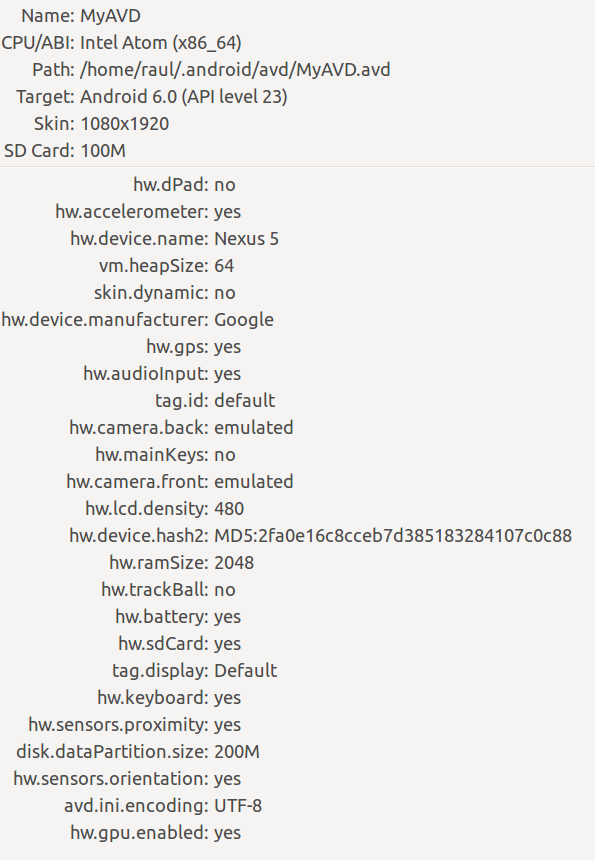
\includegraphics[width=225px]{chapter4/android-AVD_properties}
			\caption{Características del dispositivo virtual}
		    	\label{fig:chapter04:androidAVDproperties}
	\end{subfigure}
	\begin{subfigure}{.55\textwidth}
		    \centering
			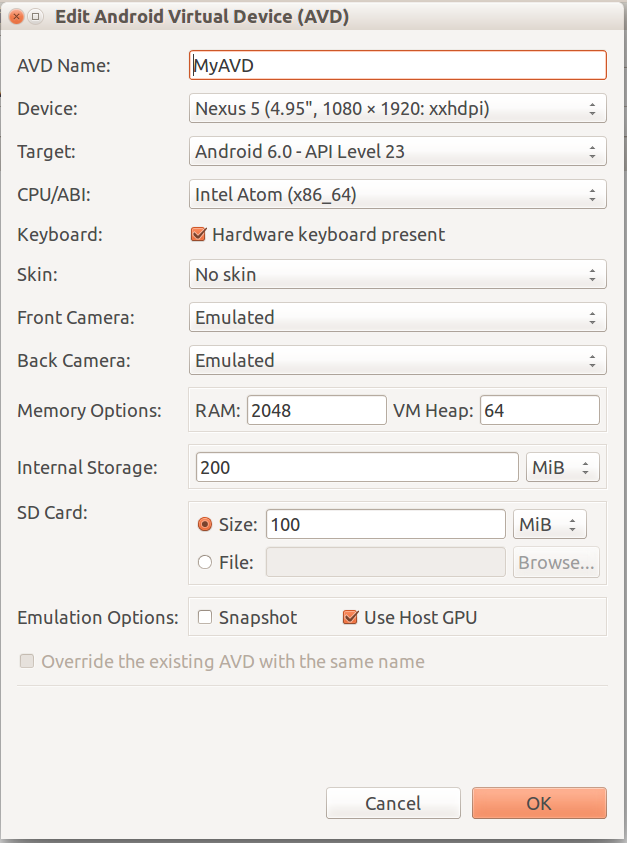
\includegraphics[width=225px]{chapter4/android-AVD_settings}
			\caption{Captura de la configuración del dispositivo virtual}
		    	\label{fig:chapter04:androidAVDsettings}
	\end{subfigure}
\end{figure}
AVD tiene las siguientes características:
\begin{itemize}
	\item 
\end{itemize}
\subsection*{IOS Simulator}
version 9.1
\textbf{explicar que es y como se configura!!!}
\begin{figure}[!pb]
		    \centering
			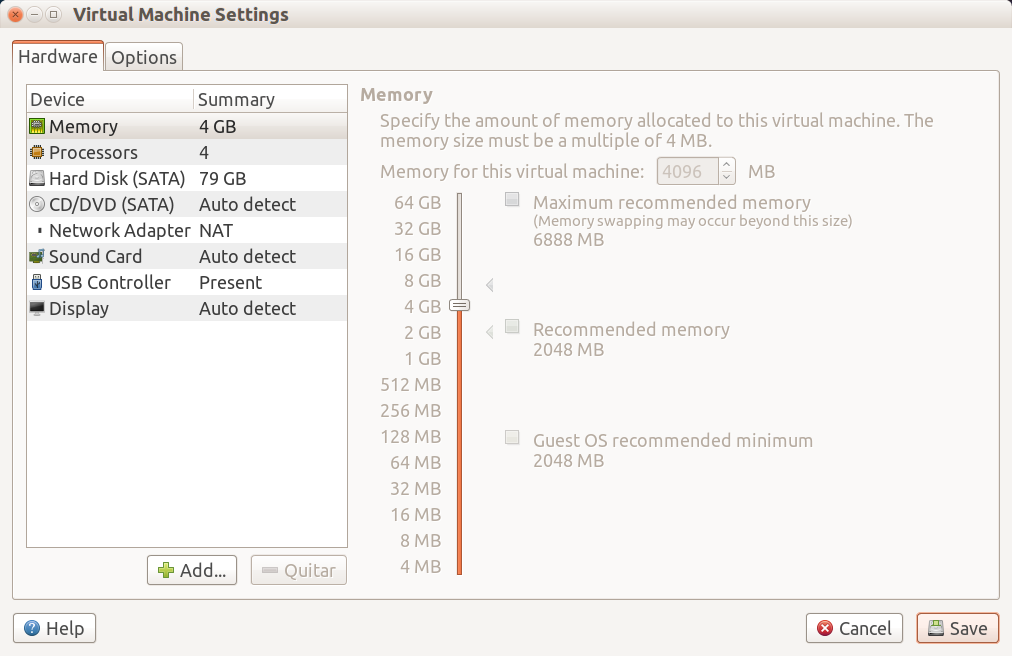
\includegraphics[width=450px]{chapter4/virtual-machine-mac}
			\caption{Características del dispositivo virtual}
		    	\label{fig:chapter04:VMwareVirtualMachine}
\end{figure}
AVD tiene las siguientes características:
\begin{itemize}
	\item 
\end{itemize}